\begin{table*}[t!]
\small
\centering
\subfloat[TPC-W]{
\begin{tabular}{|l|c|c||l|c|c|}
\hline
 Transaction name & \#paths & \#templates & Transaction name & \#paths & \#templates\\
\hline
createEmptyCart & 1 & 1 & getRelated & 1 & 0\\
doCart & 36 & 36 & getNewProducts & 1 & 0 \\
GetMostRecentOrder & 1 & 0 & createNewCustomer & 2 & 2\\
adminUpdate & 4 & 4 & getBestSellers & 1 & 0 \\
getName & 1 & 0 & doAuthorSearch & 1 & 0 \\
doSubjectSearch & 1 & 0 & GetPassword & 1 & 0\\
doTitleSearch & 1 & 0 & refreshSession & 1 & 1 \\
GetUserName & 1 & 0 & getCustomer & 1 & 0\\
getCart & 1 & 0 & doBuyConfirm-A & 32 & 32 \\
doBuyConfirm-B & 16 & 16 & getBook & 1 & 0 \\
\hline
\end{tabular}
\label{tab:staticanalysistpcwpath}
}
% \subfloat[TPC-W]{
% \centering
%  \begin{tabular}{|l|c|c||l|c|c|}
% \hline
%   Transaction name & \#paths & \#templates & Transaction name & \#paths & \#templates\\
% \hline
% read-only txns (13) & 1 & 0 &  createNewCustomer & 2 & 2 \\
% refreshSession & 1 & 1 & createEmptyCart & 1 & 1 \\
% adminUpdate & 4 & 4 & doCart & 36 & 36\\
% doBuyConfirm-A & 32 & 32 &  doBuyConfirm-B & 16 & 16\\
% \hline
%  \end{tabular}
% \label{tab:staticanalysistpcwpath}
% }

%\vspace{3mm}
\subfloat[RUBiS]{
\begin{tabular}{|l|c|c||l|c|c|}
%{|p{3.55cm}|c|c||p{2.6cm}|c|c|}%{|p{3.3cm}|c|c|}
\hline
Transaction name & \#paths & \#templates & Transaction name & \#paths & \#templates\\
\hline
ViewUserInfo & 6 & 0 & PutComment & 10 & 0\\
PutBid & 14 & 0 & BrowseRegions & 5 & 0 \\
StoreComment & 11 & 3 & StoreBid & 17 & 5 \\
BuyNow & 7 & 0 & ViewBidHistory & 11 & 0 \\
AboutMe & 37 & 0 & ViewItem & 10 & 0 \\
StoreBuyNow & 13 & 6 & RegisterItem & 59 & 24\\
SearchItemsByCategory & 20 & 0 &  BrowseCategories & 13 & 0\\       
SearchItemsByRegion & 20 & 0 & RegisterUser & 14 & 3\\
\hline
\end{tabular}
\label{tab:staticanalysisrubispath}
}

\caption{Number of reduced paths and templates generated for each transaction in TPC-W and RUBiS.}
    \label{tab:staticanalysispathreducetpcw}
\end{table*}

\subsubsection{Static analysis}
As mentioned before, taking the application source code and CRDT annotations as input, \tool\
first maps each transaction into a set of distinct paths, and automatically transforms each path into a shadow operation template. 


Table~\ref{tab:staticanalysispathreducetpcw}
summarizes the number of paths (excluding loops) and the corresponding number of shadow operation templates that were produced by \tool\ for
both TPC-W and RUBiS. For TPC-W, $15$ out of the total $20$ transactions only exhibit
a single path, as the code of these transactions is sequential. The two most complex transactions in this use case are
\texttt{doBuyConfirm} and \texttt{doCart}, which are associated with the user actions of
shopping and purchasing.
In contrast, most transactions in RUBiS have a more complex control flow,
which generated a larger number of possible execution paths. 

Note that the majority of transactions in both use cases do not lead \tool\ to
produce any template. This happens when the transactions are read-only, and therefore do not have side effects. Additionally, in TPC-W every path in an update transaction
generates a shadow operation template, since system state is always modified. However, this is 
not true in RUBiS, because its code verifies several conditions, some of which lead to a read-only transaction. 
%an abort.
\begin{table}[t!]
\centering
    \begin{tabular}{ | c | c | c | c | c | c |}
    \hline
    \multirow{2}{*}{App} & \multirow{2}{*}{\#code} & \multicolumn{2}{c|}{templates} & \multirow{2}{*}{\#db code} & \multirow{2}{*}{\#specs}\\ \cline{3-4}
       &       &  num & \#code & & \\\hline
    TPC-W & 8.3k & 92 & 1554 & 879 & 730\\
    RUBiS & 9.8k & 41 & 251 & 477 & 371\\
    \hline
    \end{tabular}
    \caption{Overview of the output produced by the static analysis. ``db code'' refers to the Java classes representing  database structures required for computing weakest preconditions.}
    \label{tab:staticanalysisoutput}
\end{table}

\begin{table}[t!]
\centering
\begin{tabular}{|c|c|c|}
\hline
 & WP & Comments \\
\hline
\multirow{2}{*}{TPC-W} & \texttt{TRUE} & Not influencing invariants \\
\cline{2-3}
& $\texttt{delta} \geq 0$ & Non-negative stock \\
\hline
\multirow{4}{*}{RUBiS} & \texttt{TRUE} & Not influencing invariants \\
\cline{2-3}
& \texttt{FALSE} & Nickname must be unique \\
\cline{2-3}
& $\texttt{delta} \geq 0$ & Non-negative quantity \\
\cline{2-3}
& $\texttt{quantity} \geq 0$ & Non-negative quantity (new item) \\
\hline
\end{tabular}
\caption{Weakest preconditions (WP)}
\label{tab:generatedwp}
\end{table}

\begin{table}[t!]
\centering
\begin{tabular}{|c|c|c|c|c|}
\hline
App & JahobSpec & Template & WP & Total \\\hline
TPC-W & 9.1 $\pm$ 0.1 & 3.8 $\pm$ 0.1 & 3.3 $\pm$ 0.1 & 16.2 $\pm$ 0.3 \\
RUBiS & 8.9 $\pm$ 0.0 & 3.3 $\pm$ 0.3 & 0.9 $\pm$ 0.1 & 13.2 $\pm$ 0.3 \\
\hline
\end{tabular}
\caption{Average and standard deviation of latency in seconds for static analysis tasks (5 runs).}
\label{tab:timestatic}
\end{table}

As depicted in Table~\ref{tab:staticanalysisoutput}, the execution
of \tool\ generated a total of $92$ and $41$ shadow operation
templates for TPC-W and RUBiS, respectively.  In addition to these
templates, our tool also generates automatically a set of Java classes
that represent database data structures, which are necessary
for computing weakest preconditions.
%%alongside specific logic conditions that are used by Jahob.

\begin{figure}[t!]
\centering
\subfloat[TPC-W]{
\centering
%\begin{minipage}[b]{0.45\textwidth}
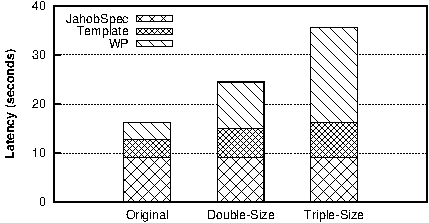
\includegraphics[width=0.66\textwidth]{./figures/sieve/eval/xytpcwanalysis.pdf}
\label{fig:tpcwtimeanalysis1}
%\end{minipage}
}
\par\bigskip
\subfloat[RUBiS]{
\centering
%\begin{minipage}[b]{0.45\textwidth}
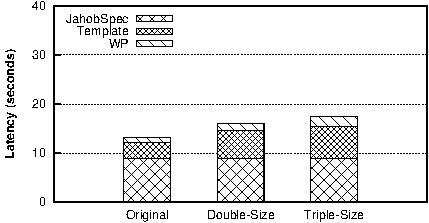
\includegraphics[width=0.66\textwidth]{./figures/sieve/eval/xyrubisanalysis.pdf}
\label{fig:rubistimeanalysis1}
%\end{minipage}
}
\caption{Static analysis time vs.\ code base size.}
\label{fig:compDiffSize}
\end{figure}

Table~\ref{tab:generatedwp} depicts a full list of the different weakest preconditions
generated by \tool\ for both use cases. These weakest preconditions alongside their 
respective shadow operation template identifiers are used by the runtime logic to classify shadow operations as either blue or red. 
A weakest precondition denoted by \texttt{TRUE} implies that any shadow operation associated
with that template is always invariant safe and therefore labeled blue.
In contrast, a weakest precondition denoted by \texttt{FALSE} implies that shadow operations
associated to that template must always be classified as red.
The remaining non-trivial conditions must be evaluated at runtime by replacing their 
arguments with concrete values. For
instance, when a \texttt{doBuyConfirm} transaction produces a negative delta, then
the condition will be evaluated to \texttt{FALSE} and the corresponding shadow operation will
be classified as red, otherwise the condition will be evaluated to \texttt{TRUE} and the 
shadow operation will be classified as blue.

\paragraph{Cost of static analysis.} A relevant aspect of the static analysis component
in \tool\ is the time required to execute it. To study this we have measured the time
taken by the static analysis and present the obtained results in Table~\ref{tab:timestatic}.
We not only measured the end-to-end completion time, but also the time
spent for each step, namely, creating database data structures required by Jahob (JahobSpec), 
template creation (Template), and weakest precondition computation (WP). 
Overall, we can see that the execution time
of the static component of \tool\ is acceptable, as less than
20 seconds are required to analyze both TPC-W and RUBiS. 
%The weakest precondition
%computation via Jahob dominates the overall static analysis time. 
The code generation phase including both JahobSpec and Template dominates
the overall static analysis. Compared to TPC-W, the time spent
computing weakest preconditions is shorter in RUBiS, due to
the smaller number of templates in Table~\ref{tab:staticanalysisoutput}.
%Compared
%to TPC-W, the time spent extracting path information in RUBiS is larger, due to
%the more complex control flow of RUBiS, as shown in Table~\ref{tab:staticanalysistpcwpath}.

%\begin{table*}[!ht]
%\footnotesize
%\centering
%\begin{tabular}{|c|c|c|c|c|c|c|}
%\hline
%App & CFG & PathAb & ReducedPathAb & Template & WP & Total \\\hline
%TPC-W & 460.5 $\pm$ 110.8 & 292.1 $\pm$ 22.2 & 365.9 $\pm$ 29.4 & 294.0$\pm$ 168.9 & 3519.6 $\pm$ 156.2 & 4932.1 $\pm$ 184.8\\
%RUBiS & 309.1 $\pm$ 75.9 & 656.0 $\pm$ 44.1 & 501.0 $\pm$ 27.2 & 248.4 $\pm$ 42.9 & 841.1 $\pm$ 41.2 & 2555.5 $\pm$ 174.0\\
%\hline
%\end{tabular}
%\caption{Average latency in milliseconds plus standard deviation for static analysis tasks (5 runs).}
%\label{tab:timestatic}
%\end{table*}

\paragraph{Scalability.} The code base size of TPC-W and RUBiS is somewhat
small when compared to deployed applications.  This raises a question
concerning the scalability of the static analysis component of
\tool\ with respect to the size of the code base. In order to analyze this aspect of \tool\ 
we have artificially doubled and tripled the size of each application
code base and measured the time spent analyzing these larger
code bases when compared with the original. The results are shown in
Figure~\ref{fig:compDiffSize}. The time spent generating the
data structures required by Jahob is constant, since we did not
change the database schema. However, the time spent
computing the weakest preconditions for templates in TPC-W grows
exponentially, and the time taken for the remaining steps presents a
sub-linear increase. These results lead us to conclude
that the static analysis of \tool\ may scale to reasonable though not very large code sizes,
especially taking into account that this process is executed a single
time when adapting an application through the use of \tool.
